%%%%%%%%%%%%%%%%%%%%%%%%%%%%%%%%%%%%%%%%%%%%%%
%%%%%%%%%%%%%%%%%%%%%%%%%%%%%%%%%%%%%%%%%%%%%%
%%			     Anexo A     			    %%
%%%%%%%%%%%%%%%%%%%%%%%%%%%%%%%%%%%%%%%%%%%%%%
%%%%%%%%%%%%%%%%%%%%%%%%%%%%%%%%%%%%%%%%%%%%%%
\appendix
\chapter{Pruebas con ``Reactor''} \label{anexoA}
\newpage

Para comprender mejor el funcionamiento de esta biblioteca, a continuación se exponen un conjunto de ejemplos que tratan distintos tipos de eventos: eventos de entradas digitales, eventos de carácter periódico, eventos de parpadeo de un led y eventos de programas externos.

\begin{itemize}
    \item Eventos de entradas digitales
    
    En este proyecto, se usa el manejador ``event\_hanlder'' para tratar eventos procedentes de un teclado y un ratón, sin embargo, los eventos pueden proceder de botones asignados a las patillas GPIO de Raspberry Pi. 
    
    \begin{figure}[H]
    \centering
    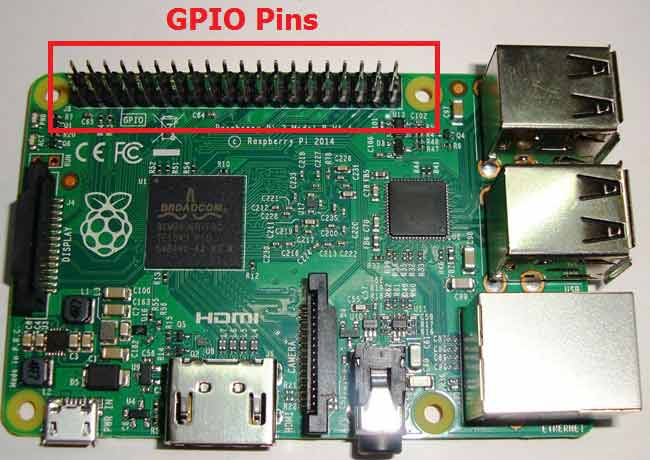
\includegraphics[scale = 0.3]{anexo_a/figuras_dir/GPIO.jpg}
    \caption{Pines GPIO de Raspberry Pi 3 modelo B}
    %\label{fig:figura4}
    \end{figure}
    
    El programa siguiente procesa los eventos de los pines GPIO asignados como entradas digitales:
    
\begin{listing}
\begin{minted}[bgcolor=bg,
               frame=lines,
               framesep=2mm,
               linenos]
               {C}

#include <reactor/reactor.h>
#include <reactor/input_handler.h>
#include <stdio.h>
#include <wiringPi.h>


static void press(input_handler* ev, int key) { printf("Press %d\n", key);}
static void release(input_handler* ev, int key) {printf("Release %d\n", key); }

int main ()
{
	
	int buttons[]= {10,23,24};
	wiringPiSetupGpio();
	reactor* r= reactor_new();
	reactor_add(r, (event_handler*) input_handler_new(buttons, 4, press, release));
	
	reactor_run(r);
	
	
}


\end{minted}
\caption{Programa de eventos de entradas digitales}
\label{prg:digital-input-events}
\end{listing}
    

En este caso, se usa otro manejador denominado ``input\_handler''. En este ejemplo, se declara en un vector los pines GPIO que constituyen la fuente de eventos. Posteriormente, se inicializa la biblioteca ``WiringPi'' con la función ``wiringPiSetupGpio()'' que permite que el programa tenga acceso a los pines GPIO mediante el esquema de enumeración de pines de esta biblioteca. A continuación, se crea un objeto de tipo ``reactor'' sobre el que se registra el manejador. Finalmente, se inicia el bucle de eventos.

Tras ejecutarlo con el mismo archivo ``makefile'' usado en el programa de demultiplexado de eventos, el terminal muestra las entradas cuyos botones son pulsados (press) y soltados (release).

    \begin{figure}
    \centering
    \includegraphics[scale = 0.05]{anexo_a/figuras_dir/montaje1.jpg}
    \caption{Montaje de programa de eventos de entradas digitales}
    %\label{fig:figura4}
    \end{figure}

    
    \begin{figure}[htbp]
    \centering
    \subfigure[Entrada 10]{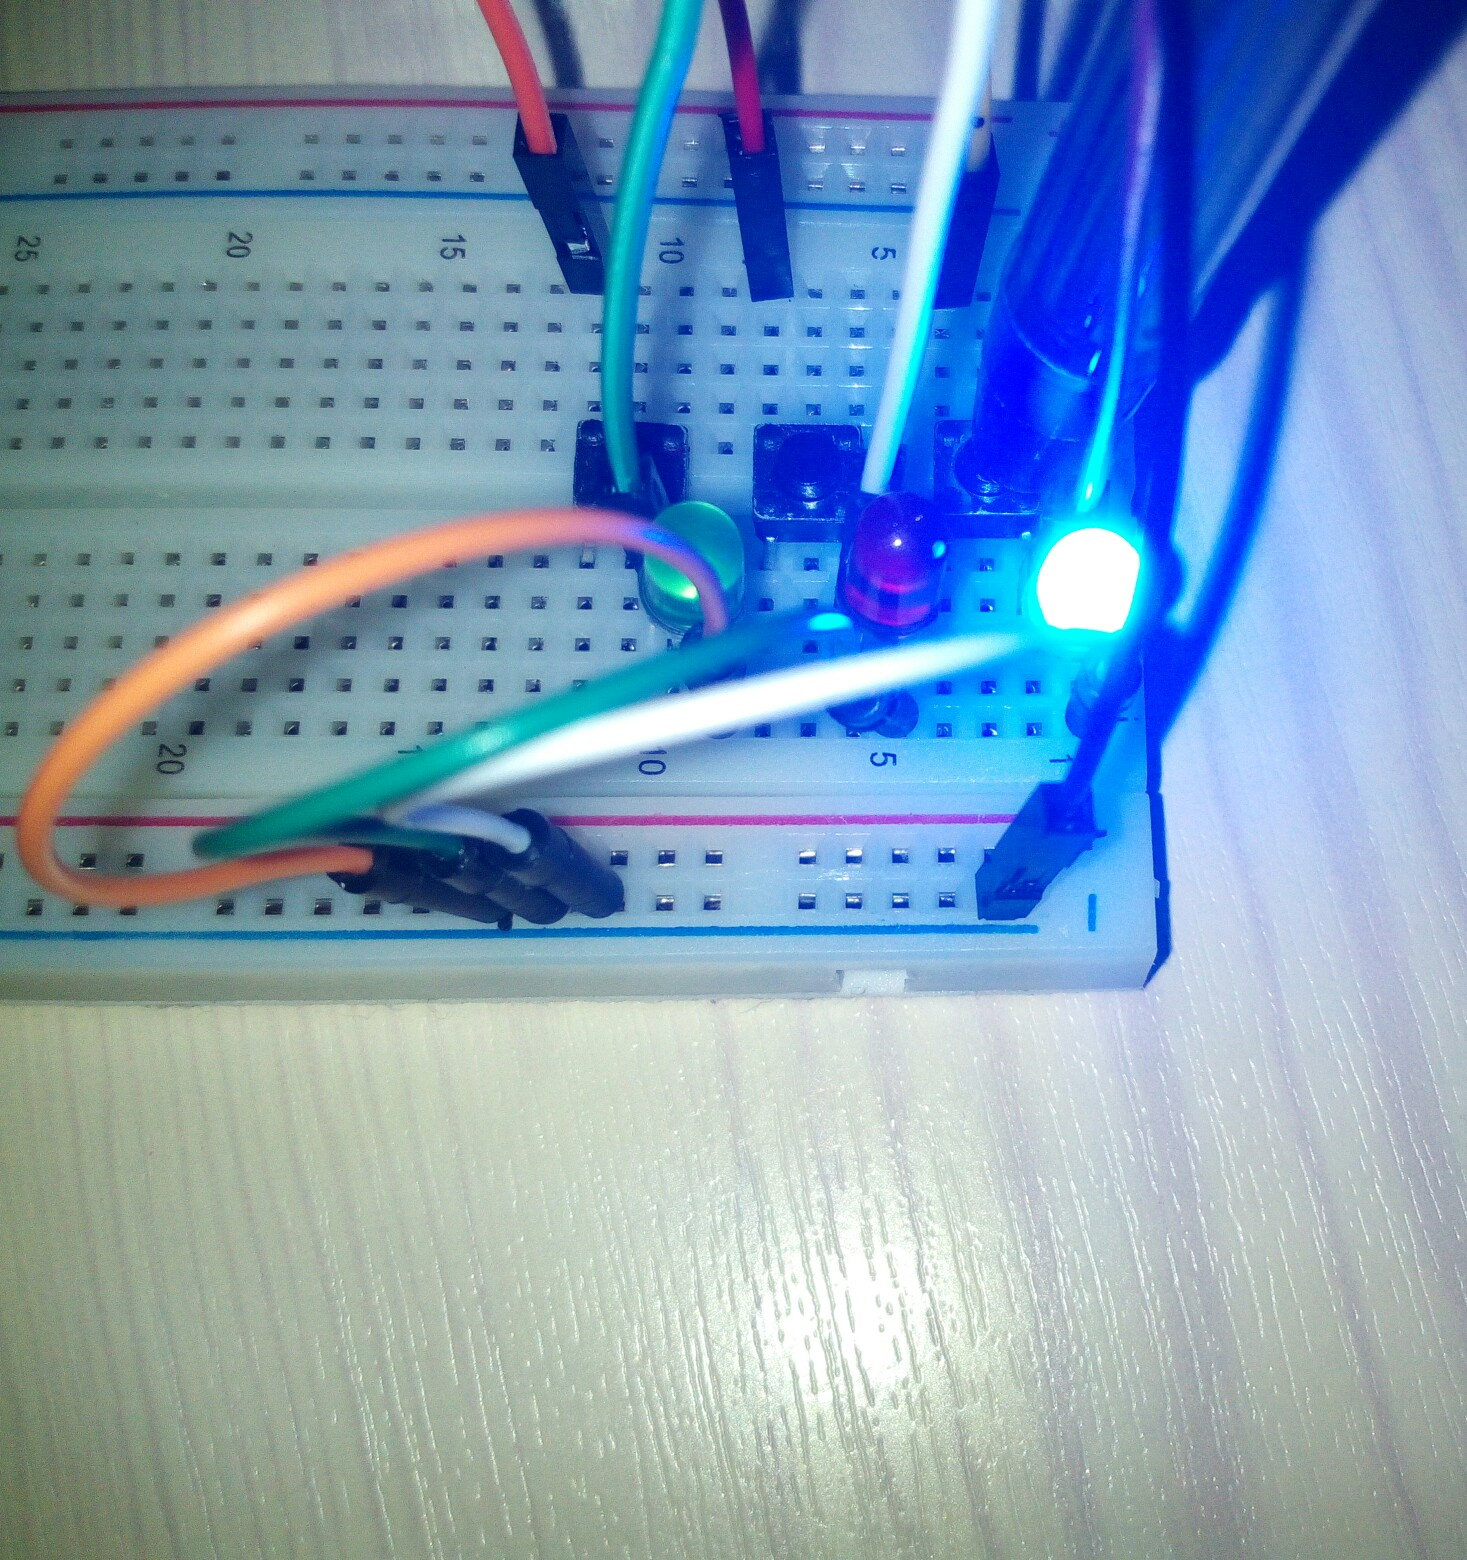
\includegraphics[width=50mm, height=50mm]{anexo_a/figuras_dir/ent10.jpg}}
    \subfigure[Entrada 23]{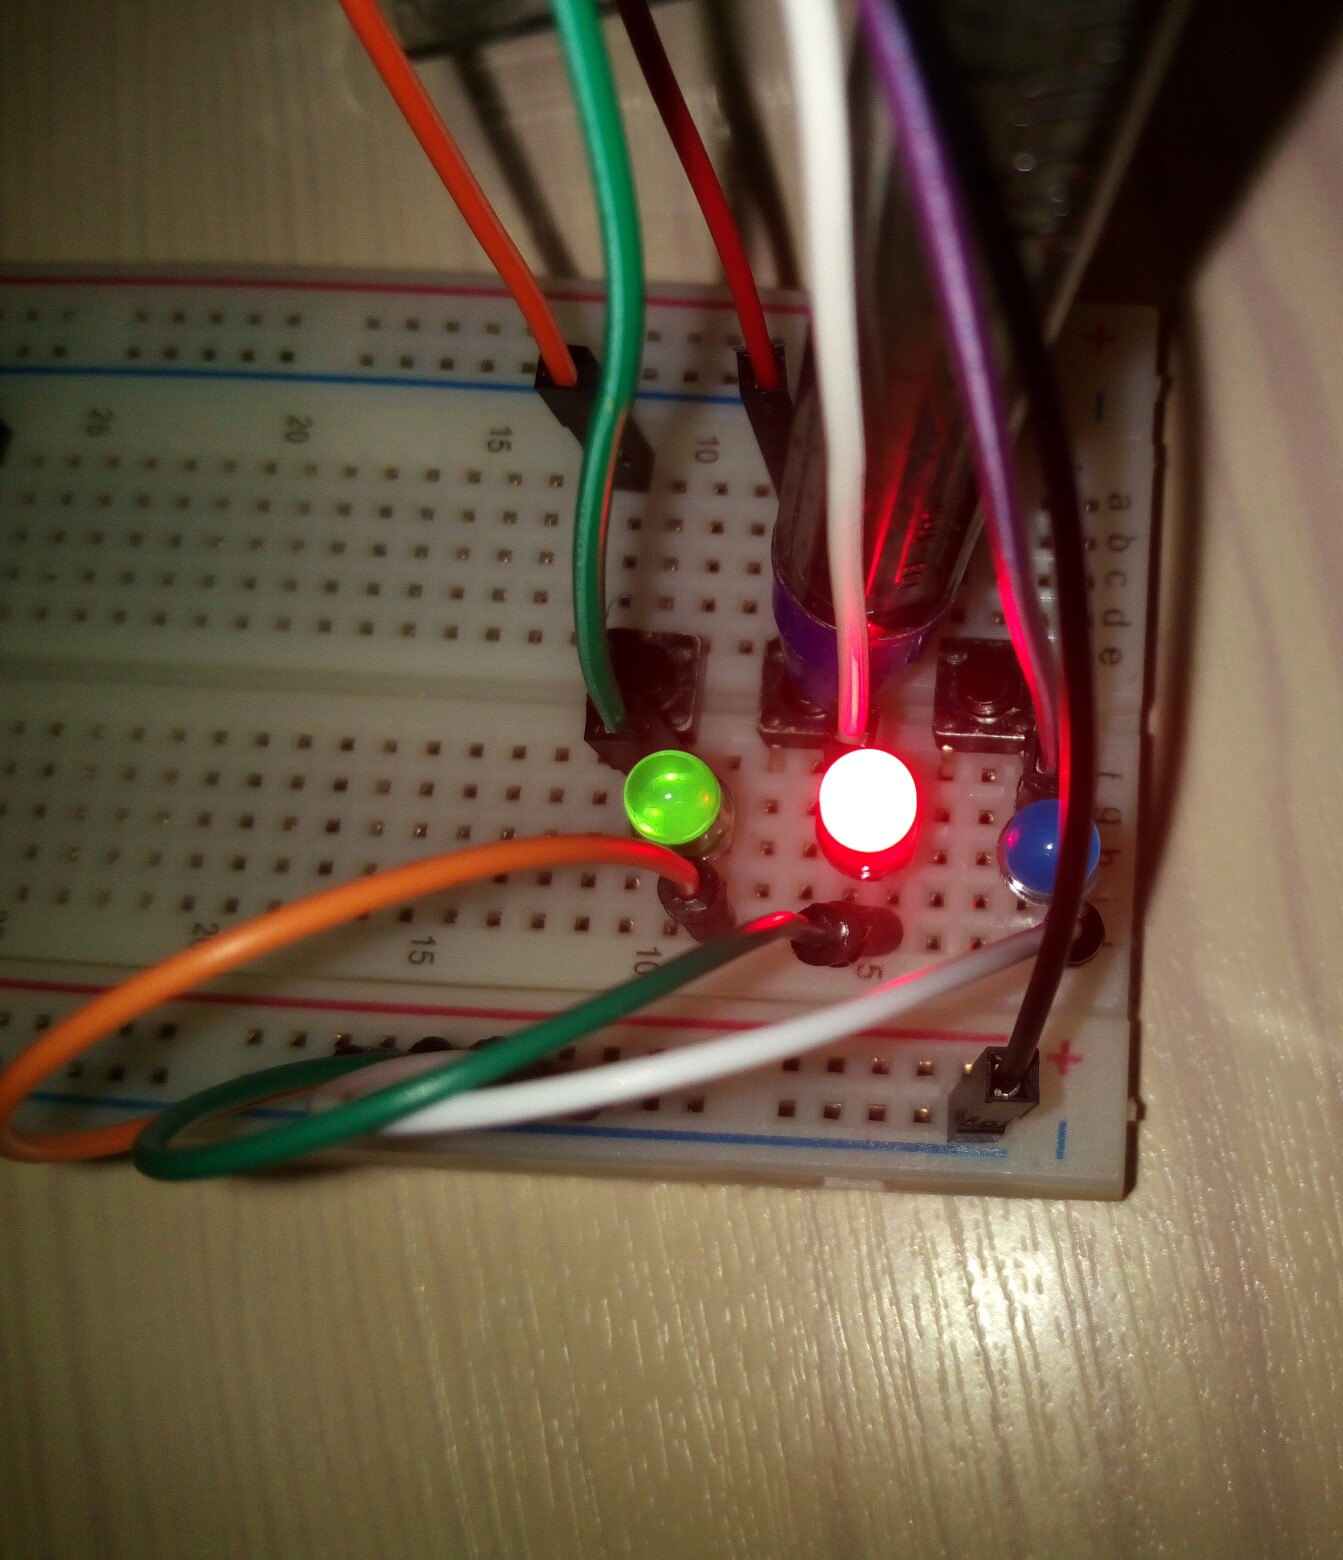
\includegraphics[width=50mm, height=50mm]{anexo_a/figuras_dir/ent23.jpg}}
    \subfigure[Entrada 24]{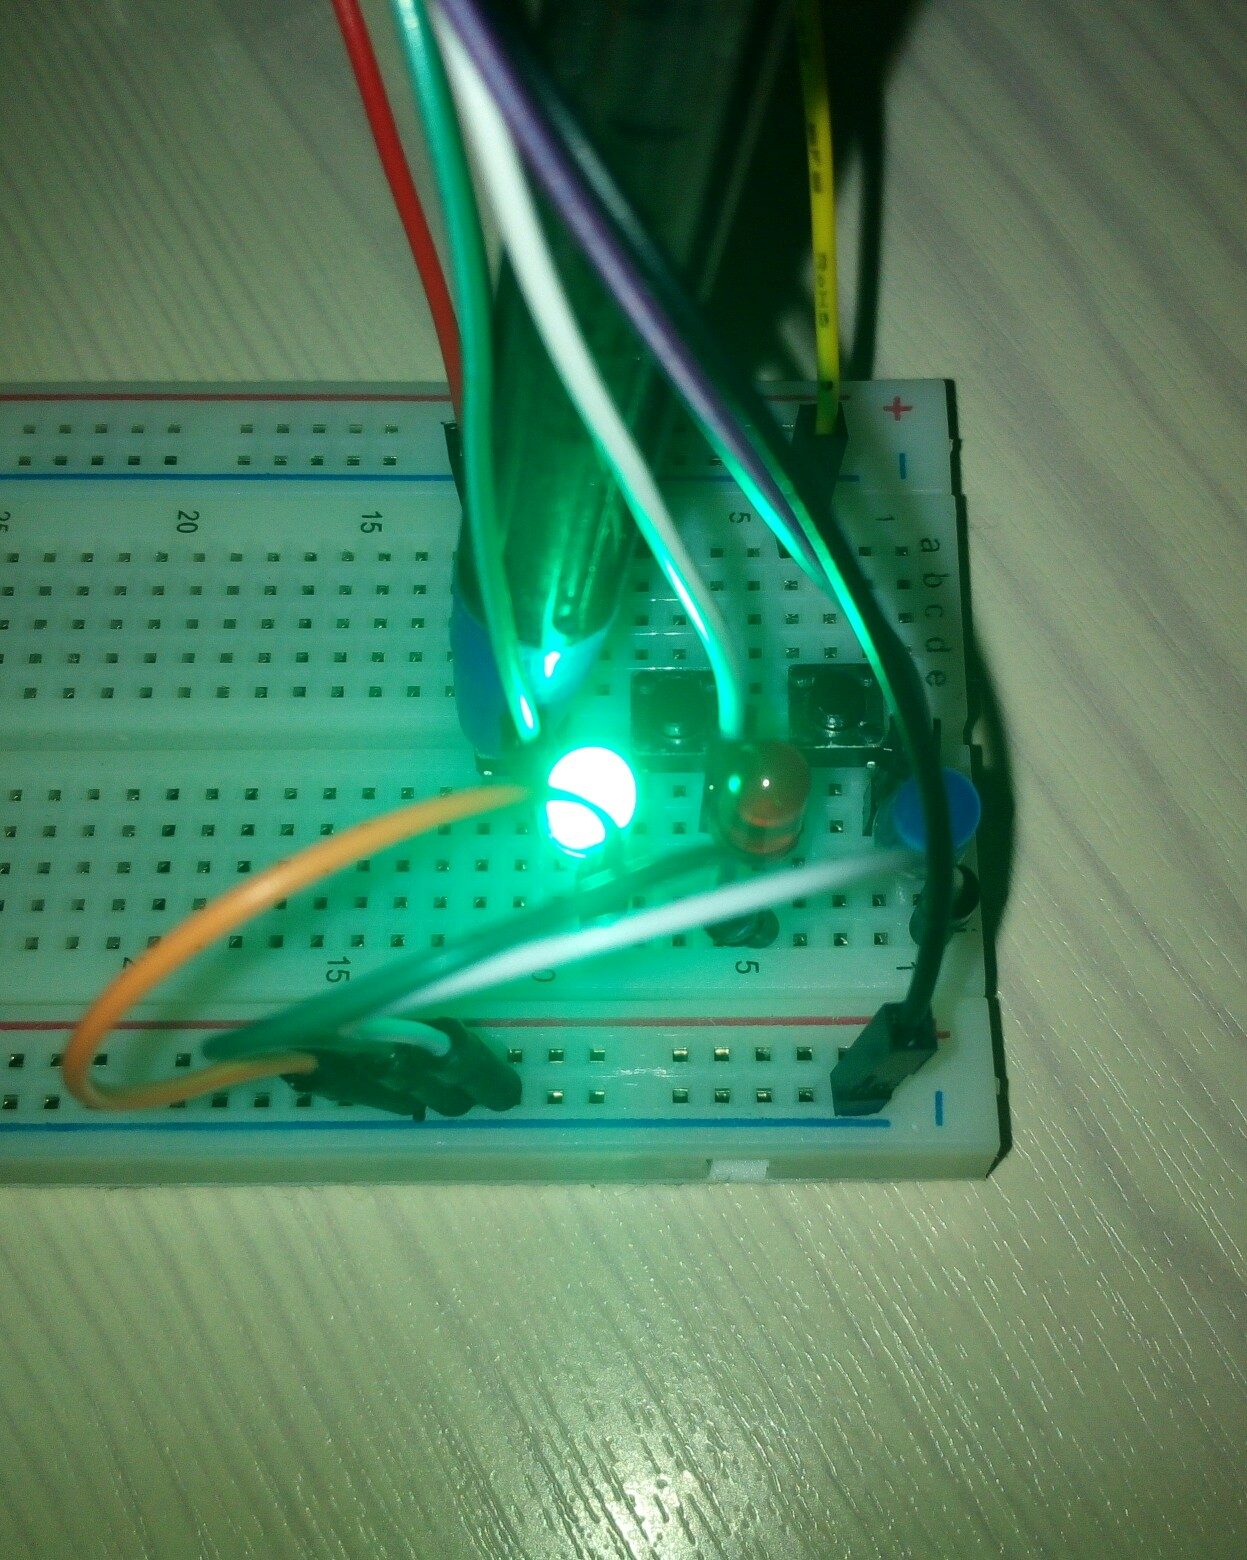
\includegraphics[width=50mm, height=50mm]{anexo_a/figuras_dir/ent24.jpg}}
    \caption{Pulsaciones de los botones de las entradas 10, 23 y 24 GPIO}
    %\label{fig:lego}
    \end{figure}
    
    \begin{figure}
    \centering
    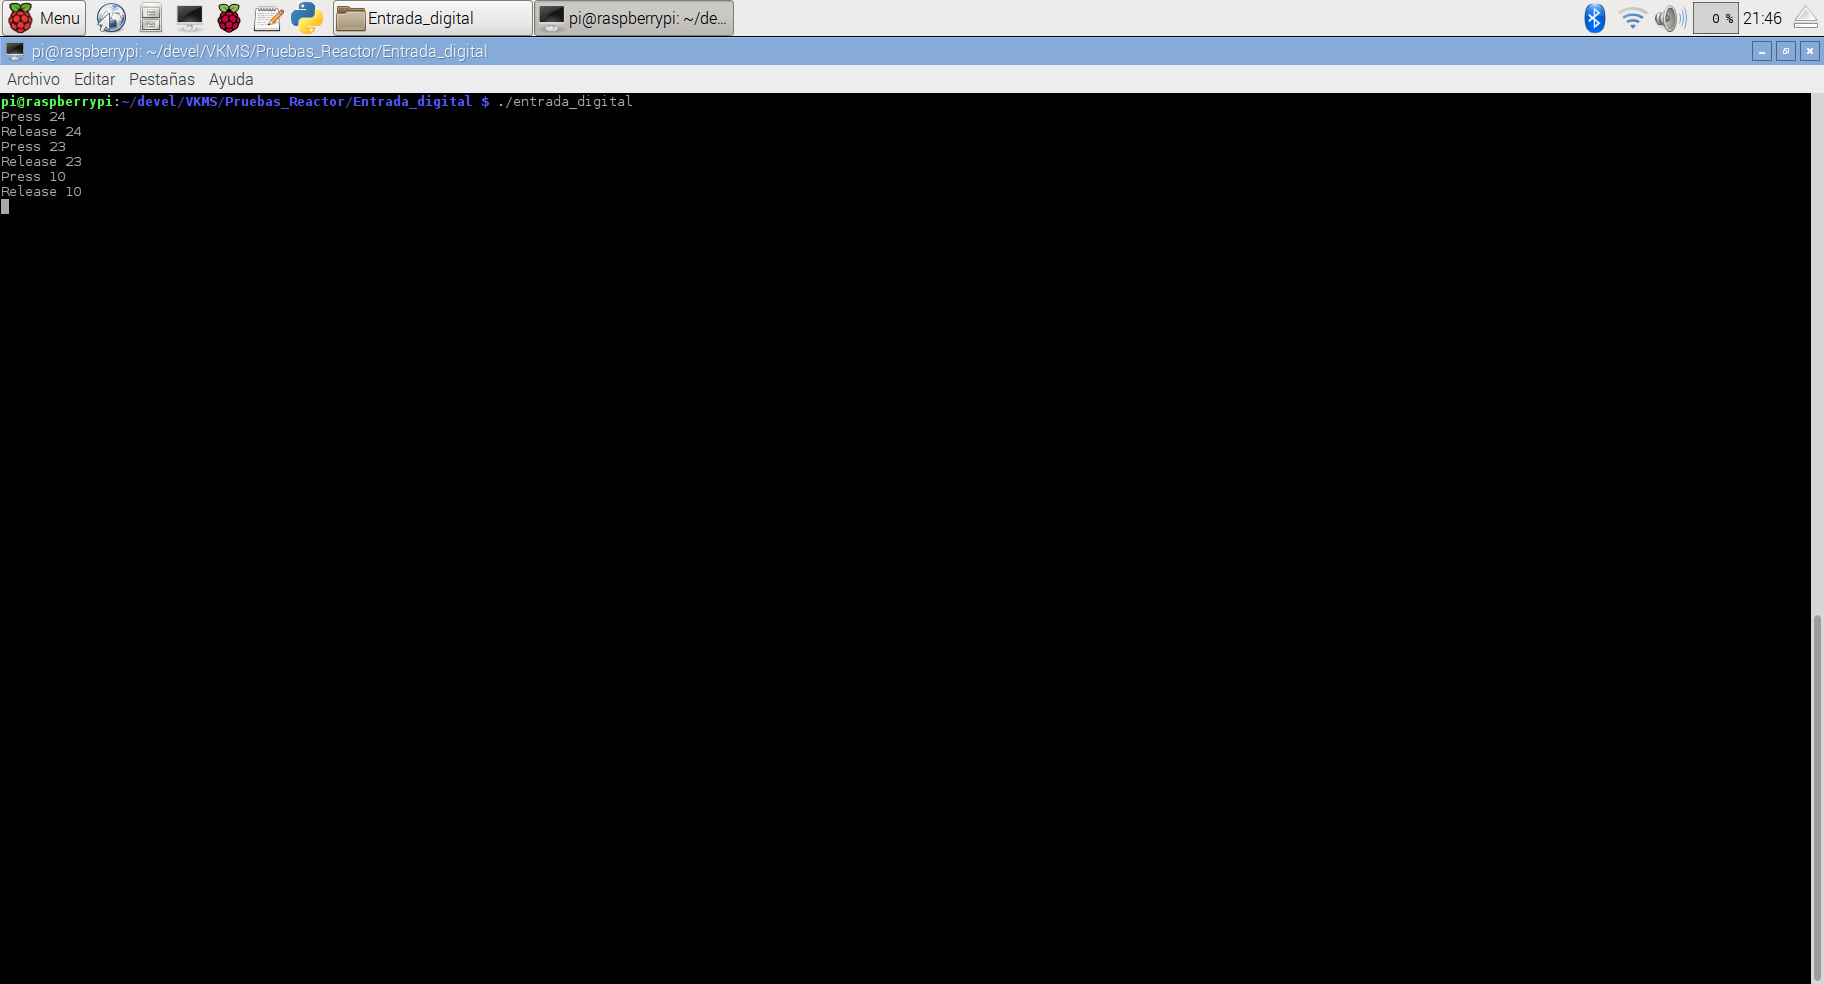
\includegraphics[scale = 0.25]{anexo_a/figuras_dir/res1.jpg}
    \caption{Salida del programa de eventos de entradas digitales}
    %\label{fig:figura4}
    \end{figure}

\clearpage

    \item Eventos periódicos
    
    El programa de este ejemplo, genera eventos cada cierto tiempo fijo en un descriptor especial que son procesados por un nuevo manejador: ``periodic\_handler''. 
    
\begin{listing}
\begin{minted}[bgcolor=bg,
               frame=lines,
               framesep=2mm,
               linenos]
               {C}

#include <reactor/reactor.h>
#include <reactor/periodic_handler.h>
#include <reactor/exception.h>
#include <stdio.h>

void handler(event_handler* ev) 
{
	puts("Tick");
}

int main () 
{
	reactor* r= reactor_new();
	reactor_add(r, (event_handler*)periodic_handler_new(2000, handler));
	reactor_run(r);
	return 0;
}

\end{minted}
\caption{Programa de eventos periódicos}
\label{prg:periodic-events}
\end{listing}

    
    La parte principal (``main()''), funciona de la misma forma que el anterior, sin embargo, en lugar de imprimir los cambios en los niveles lógicos de las entradas, imprime el evento que genera cada 2 segundos (2000 milisegundos), que en este caso, es el mensaje mostrado entre comillas.

    \begin{figure}[htbp]
    \centering
    \subfigure[Mensajes de eventos en t=t1]{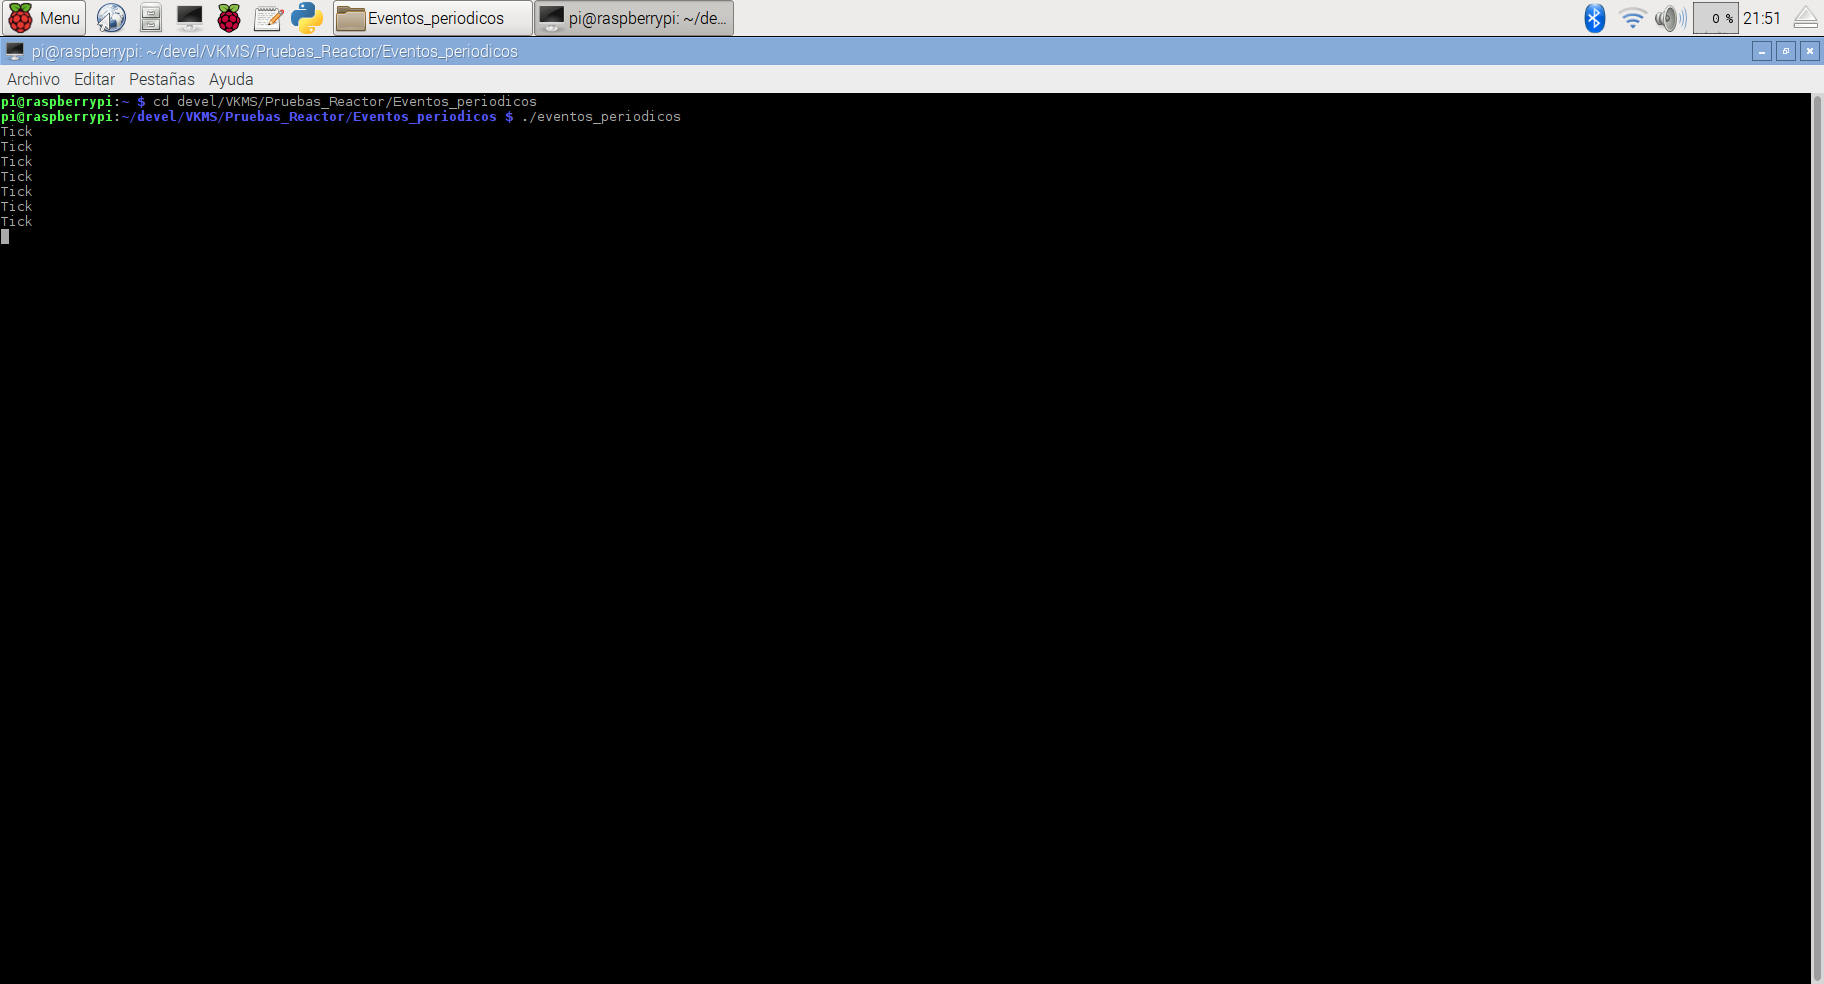
\includegraphics[width=90mm, height=70mm]{anexo_a/figuras_dir/res2.jpg}}
    \subfigure[Mensajes de eventos en t=t2]{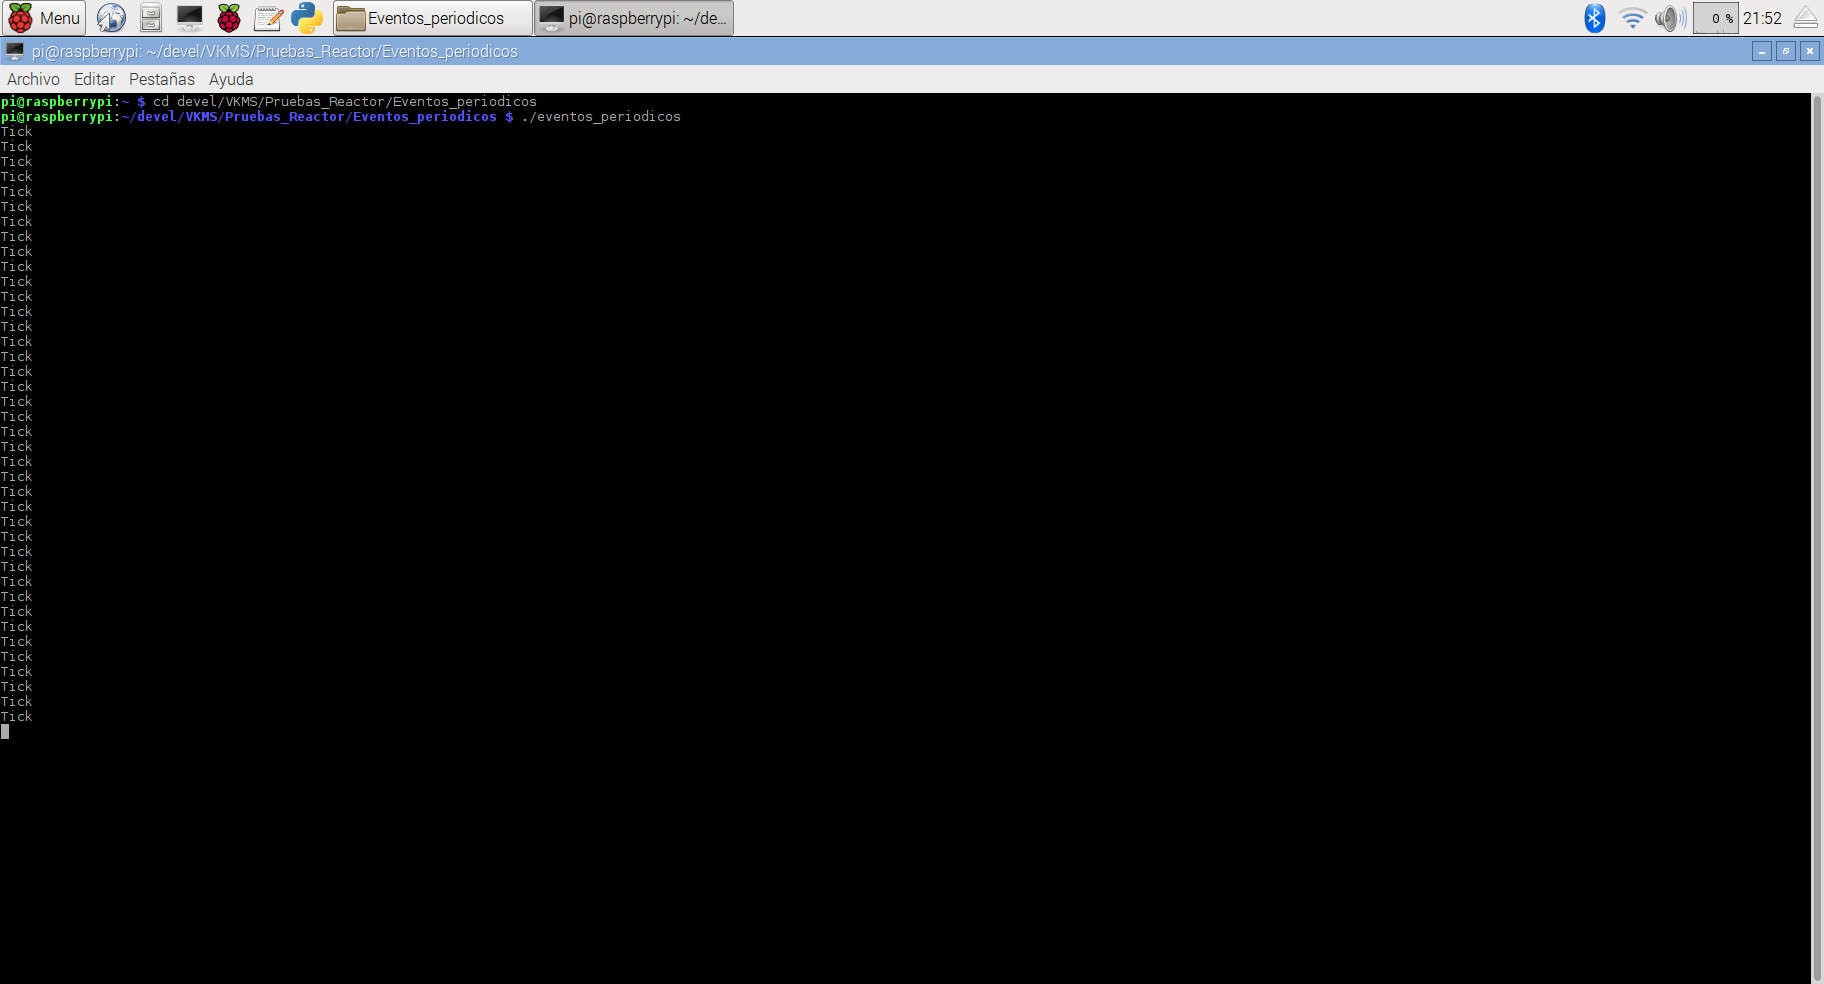
\includegraphics[width=90mm, height=70mm]{anexo_a/figuras_dir/res3.jpg}}
    \caption{Salida del programa de eventos periódicos en t=t1 y t=t2 siendo t1<t2}
    %\label{fig:lego}
    \end{figure}

\clearpage
    \item Parpadeo de un led
    
    Este programa envía cada cierto tiempo un pulso de corriente a un led conectado a una de los pines GPIO con un número determinado de milisegundos de duración que se repite tantas veces como ciclos de encendido/apagado se especifiquen.
    
\begin{listing}
\begin{minted}[bgcolor=bg,
               frame=lines,
               framesep=2mm,
               linenos]
               {C}

#include <reactor/reactor.h>
#include <reactor/blink_handler.h>
#include <wiringPi.h>
#include <stdio.h>

int main ()
{
	wiringPiSetupGpio();
	reactor* r= reactor_new();
	reactor_add(r, (event_handler*) blink_handler_new(18, 200, 5));
	reactor_run(r);
	
}

\end{minted}
\caption{Programa de parpadeo de un led}
\label{prg:led-blink}
\end{listing}
    
    Cuando se llama al constructor del manejador (``blink\_handler'') se deben indicar los tres argumentos referidos al pin GPIO, al tiempo de encendido y apagado y al número de ciclos respectivamente.
    
    \begin{figure}[htbp]
    \centering
    \subfigure[Led del pin 18 a nivel bajo]{\includegraphics[width=50mm, height=50mm]{anexo_a/figuras_dir/led1.jpg}}
    \subfigure[Led del pin 18 a nivel alto]{\includegraphics[width=50mm, height=50mm]{anexo_a/figuras_dir/led2.jpg}}
    \caption{Parpadeo del led del pin 18}
    %\label{fig:lego}
    \end{figure}
\clearpage
    \item Eventos de programas externos
    
    El manejador ``music\_player'' ejecuta un programa ajeno al principal. Se trata de ``mpg123'' que se usa para reproducir música en formato ``.mp3''.
\begin{listing}[p]
\begin{minted}[bgcolor=bg,
               frame=lines,
               framesep=2mm,
               linenos]
               {C}
#include <reactor/reactor.h>
#include <reactor/console.h>
#include <reactor/music_player.h>
#include <stdio.h>
#include <unistd.h>


static int read_key(int fd);

int main (int argc, char* argv[])
{
	const  char* carpeta = "/usr/share/scratch/Media/Sounds/Music Loops";
	void* state = console_set_raw_mode(0);
	reactor* r = reactor_new();
	music_player* mp = music_player_new(carpeta);
	
	void keyboard(event_handler* ev) {
		int key = read_key(ev->fd);
		if ('q' == key)
		reactor_quit(r);
		else if (' ' == key)
		music_player_stop(mp);
		else if (key >= '0' && key <= '9')
		music_player_play(mp, key - '0');
	}
	
	reactor_add(r, (event_handler*)mp);
	reactor_add(r, event_handler_new(0, keyboard));
	reactor_run(r);
	reactor_destroy(r);
	console_restore(0, state);
}

static int read_key(int fd)
{
	char buf[2];
	if (0 < read(fd, buf, 1))
	return buf[0];
	return -1;
}
\end{minted}
\caption{Programa de reproducción de música}
\label{prg:mp3-player}
\end{listing}

    
    En primer lugar, se declara e inicializa una cadena de caracteres con la ruta de los archivos ``.mp3''' a reproducir. Seguidamente, se construye un manjeador ``music\_player'' cuyo argumento es el directorio anterior. Después, se crea la función ``keyboard()'' que lee el descriptor registrado mediante ``read\_keyboard()'' en el manejador ``event\_hanlder'' que se crea posteriormente y define el comportamiento del programa cuando se pulsan un conjunto de teclas:
    
    \begin{itemize}
        \item Si se pulsa ``q'' el bucle de eventos finaliza, y por tanto, también el programa.
        \item Si se pulsa la tecla ``espacio'' se llama a ``music\_player\_stop()'' que interrumpe la reproducción de la música.
        \item Si se pulsan las teclas numéricas entre los valores 0 y 9 (inclusives), ``mpg123'' reproduce la canción correspondiente.
    \end{itemize}
    
    \begin{figure}[H]
    \centering
    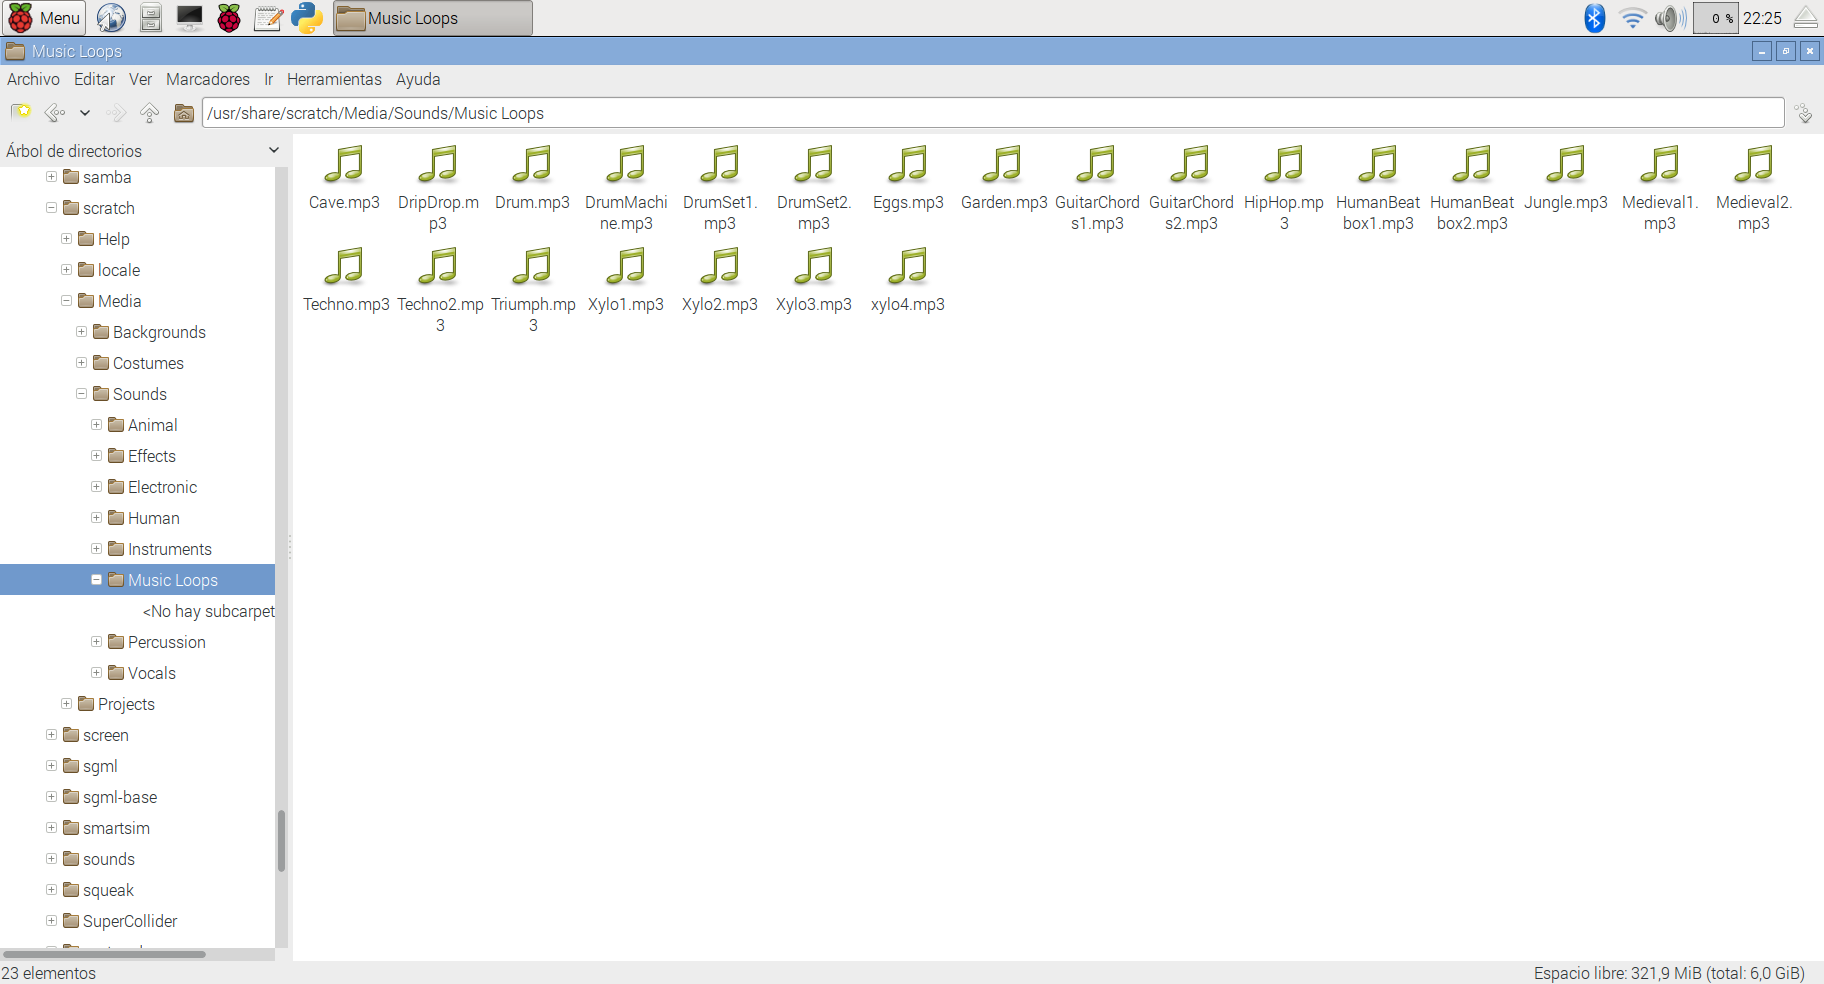
\includegraphics[scale = 0.25]{anexo_a/figuras_dir/musica.jpg}
    \caption{Canciones que se reproducen con ``mpg123''}
    %\label{fig:figura4}
    \end{figure}
  
\end{itemize}
